\documentclass[12pt]{article}
 
\usepackage[margin=1in]{geometry} 
\usepackage{amsmath,amsthm,amssymb,amsfonts}
\usepackage{color}
\usepackage{graphicx}
\graphicspath{ {Images/} }
\usepackage{float}
\setlength{\parskip}{1em}
\usepackage{cancel}
\usepackage{longtable}
\usepackage{pgf,tikz,pgfplots}
\pgfplotsset{compat=1.15}
\usepackage{mathrsfs}
\usetikzlibrary{arrows}
\pagestyle{empty}
\pagestyle{empty}
\begin{document}

\section*{Problem 4}

Problem 4 revisits Problem 2, where the optimisation problem was unconstrained and had one shared variable. Recall that the dual function was given by
\begin{align*}
q(\lambda)&=q_1(\lambda)+q_2(\lambda)\\
&=\inf_{x,\xi_1}[f_1(x,\xi_1)-\lambda\xi_1]+\inf_{y,\xi_2}[f_2(y,\xi_2)+\lambda\xi_2].
\end{align*}
Dual decomposition and the subgradient method were applied to solve this problem, where we iteratively use a given $\lambda$ to solve two separate sets of linear equations, $A_1v_1=B_1$ and $A_2v_2=B_2$, and obtain $\xi_1$ and $\xi_2$, then use $\xi_1$ and $\xi_2$ to update $\lambda$.

Consider now three agents Agent 1, Agent 2 and Agent 3. Agent 3 computes the updates $\lambda=\lambda-\alpha(\xi_1-\xi_2)$, then sends $\lambda$ to both Agent 1 and 2. Agents 1 and 2 respectively solve $A_1x_1=B_1$ and $A_2x_2=B_2$, then send $\xi_1$ and $\xi_2$ to Agent 3. This is repeated for some specified number of iterations. The figure below shows one iteration of this.

\begin{figure}[H]
	\centering
	\definecolor{rvwvcq}{rgb}{0.08,0.4,0.7}
	\begin{tikzpicture}[line cap=round,line join=round,>=triangle 45,x=1cm,y=1cm]
	\draw [line width=1pt] (-8,4) circle (0.7cm);
	\draw [line width=1pt] (-3,4) circle (0.7cm);
	\draw (-10.5,5.5) node[anchor=north west] {1) Agent 3: Updates $\lambda$};
	\draw [line width=1pt] (-7,4.5)-- (-4,4.5);
	\draw [line width=1pt] (-4,4)-- (-7,4);
	\draw [line width=1pt] (-8,1) circle (0.7cm);
	\draw [line width=1pt] (-8.3,3)-- (-8.3,2);
	\draw [line width=1pt] (-7.7,2)-- (-7.7,3);
	\draw (-3.6,5.5) node[anchor=north west] {3) Agent 1: Solves $A_1x_1+B_1=0$};
	\draw (-9,0) node[anchor=north west] {3)Agent 2: Solves $A_2x_2+B_2=0$};
	\draw (-6,5.2) node[anchor=north west] {2) Send $\lambda$};
	\draw (-6,3.9) node[anchor=north west] {4) Send $\xi_1$};
	\draw (-7.5,2.7) node[anchor=north west] {4) Send $\xi_2$};
	\draw (-10.5,2.7) node[anchor=north west] {2) Send $\lambda$};
	\begin{scriptsize}
	\draw [fill=rvwvcq,shift={(-4,4.48)},rotate=270] (0,0) ++(0 pt,3.75pt) -- ++(3pt,-6pt)--++(-6.5pt,0 pt) -- ++(3pt,5.5pt);
	\draw [fill=rvwvcq,shift={(-7,4)},rotate=90] (0,0) ++(0 pt,3.75pt) -- ++(3pt,-6pt)--++(-6.5pt,0 pt) -- ++(3pt,5.5pt);
	\draw [fill=rvwvcq,shift={(-8.3,2)},rotate=180] (0,0) ++(0 pt,3.75pt) -- ++(3pt,-6pt)--++(-6.5pt,0 pt) -- ++(3pt,5.5pt);
	\draw [fill=rvwvcq,shift={(-7.7,3)},rotate=0] (0,0) ++(0 pt,3.75pt) -- ++(3pt,-6pt)--++(-6.5pt,0 pt) -- ++(3pt,5.5pt);
	\end{scriptsize}
	\end{tikzpicture}
	\caption{Steps 1, 2, 3, 4 show the procedure in a single iteration of the subgradient method.}
\end{figure}

Previously, messages were assumed to have unlimited size, i.e., there is no floating point error when $\lambda$, $\xi_1$ and $\xi_2$ are sent between Agents 1, 2 and 3. Let's now consider a limit on message size. Assume messages are sent in binary, then there is a limit on the number of bits that can be sent.

\subsection*{Word Limit}

The following terms will be used to describe a binary number.
\begin{center}
	$\underbrace{\pm}_{\text{sign}}\underbrace{10101010101010}_{\text{binary integer}}\underbrace{.}_{\text{binary point}}\underbrace{1010101010101010}_{\text{binary fraction}}$
\end{center}


For the example problems generated, it so happens that the variable $\lambda$ is in general larger than $\xi_1$ and $\xi_2$. Messages involving $\lambda$ require at least 3 binary integer bits, while messages involving $\xi_1$ and $\xi_2$ generally have a binary integer of 0, i.e., they converge to values with absolute values smaller than 1.

Let's vary the limit on the number of bits used to represent the binary fraction, and assume the number of bits used to represent the binary integer is limited to 3 bits plus 1 bit for the sign. Thus, the word limit referred to below is the limit on the number of bits used to represent the binary fraction of a message, not including the sign and integer bits.

\subsection*{Convergence}

In order to measure convergence, we need a benchmark. Recall from Problem 2 the combined problem, where $A_1$ and $A_2$ are overlapped to form $A$, and $B_1$ and $B_2$ overlapped to form $B$. The combined problem $Av+B=0$ can be solved, and we can use the vector $v$ as a benchmark to measure convergence. Let $v^*$ be the solution to the problem $Av+B=0$, let $v_1^*$ be the solution to the problem $A_1v_1+B_1=0$ and let $v_1^*$ be the solution to the problem $A_2v_2+B_2=0$. The dimensions do not match, so let's overlap $v_1^*$ and $v_2^*$

\begin{figure}[H]
	\centering
	\definecolor{rvwvcq}{rgb}{0.08,0.4,0.7}
	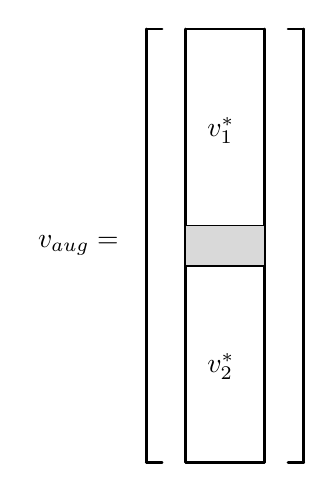
\begin{tikzpicture}[line cap=round,line join=round,>=triangle 45,x=1cm,y=1cm]
	\draw [line width=1pt] (9.5,10)-- (9.5,4.5);
	\draw [line width=1pt] (9.5,10)-- (9.7,10);
	\draw [line width=1pt] (9.7,4.5)-- (9.5,4.5);
	\draw [line width=1pt] (11.5,10)-- (11.5,4.5);
	\draw [line width=1pt] (11.3,10)-- (11.5,10);
	\draw [line width=1pt] (11.3,4.5)-- (11.5,4.5);
	\draw [line width=1pt] (10,10)-- (10,7);
	\draw [line width=1pt] (10,7)-- (11,7);
	\draw [line width=1pt] (11,7)-- (11,10);
	\draw [line width=1pt] (11,10)-- (10,10);
	\draw [line width=1pt] (10,7.5)-- (10,4.5);
	\draw [line width=1pt] (10,4.5)-- (11,4.5);
	\draw [line width=1pt] (11,4.5)-- (11,7.5);
	\draw [line width=1pt] (11,7.5)-- (10,7.5);
	\draw[fill=gray!30]    (11,7) -- (11,7.5) -- (10,7.5) -- (10,7);
	\draw (10.15,9) node[anchor=north west] {$v_1^*$};
	\draw (10.15,6) node[anchor=north west] {$v_2^*$};
	\draw (8,7.5) node[anchor=north west] {$v_{aug}=$};
	\end{tikzpicture}
	\caption{Create $v_{aug}$, a vector with $v_1^*$ and $v_2^*$ overlapping as shown. Only one element is in the grey overlapping region, and that element is equal to the \textbf{mean} of the elements of $v_1^*$ and $v_2^*$ that overlap.}
\end{figure}

Finally, our measure of convergence will be $||x_{aug}-x^*||_2$.

\begin{figure}[H]
	\centering
	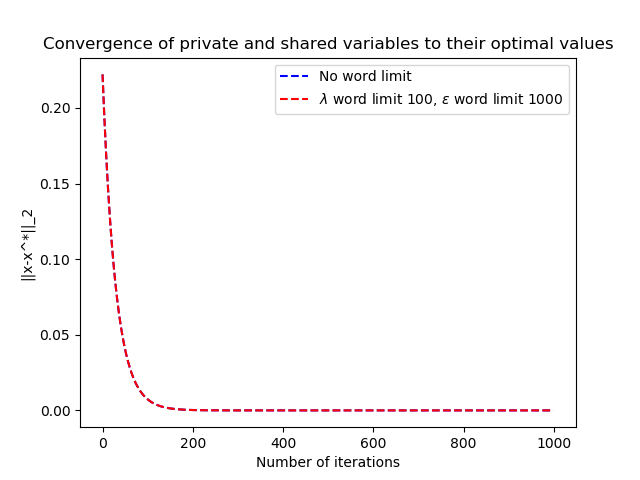
\includegraphics[scale=0.5]{Problem4-Convergence1.png}
	\caption{Large word limits.}
\end{figure}

\begin{figure}[H]
	\centering
	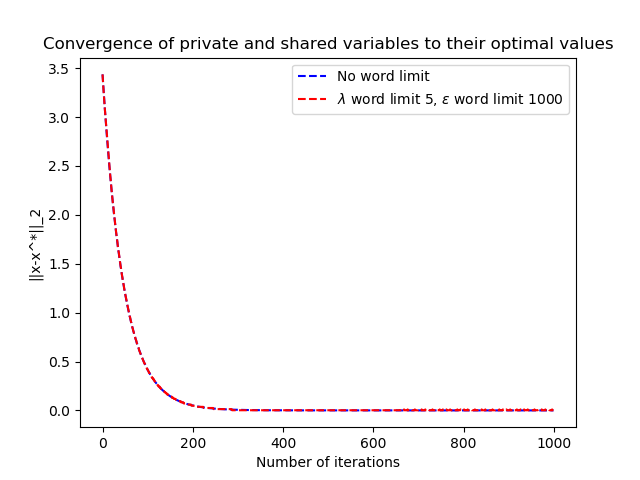
\includegraphics[scale=0.5]{Problem4-Convergence2.png}
	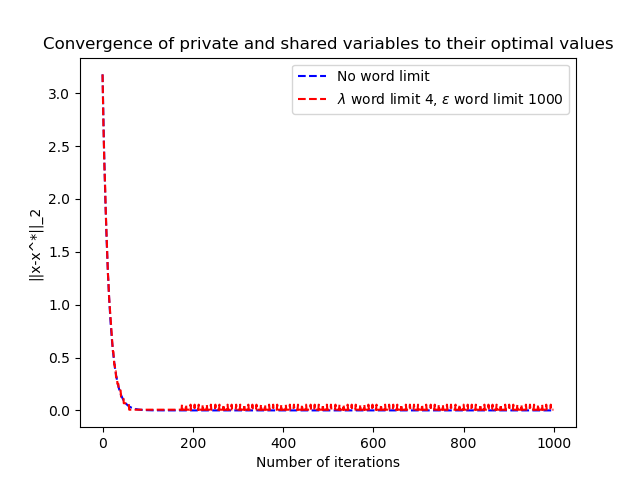
\includegraphics[scale=0.5]{Problem4-Convergence3.png}
	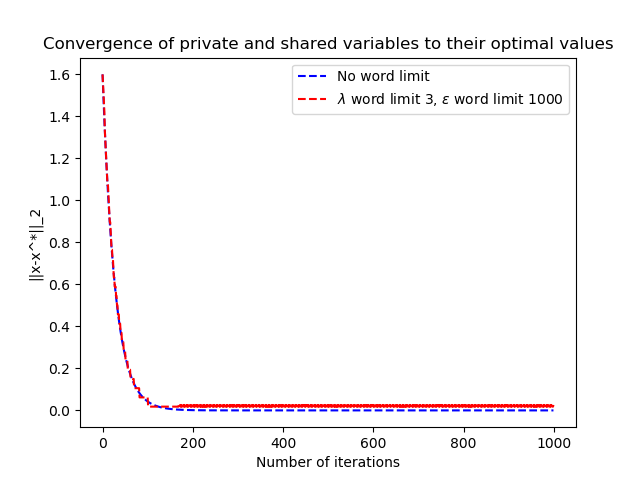
\includegraphics[scale=0.5]{Problem4-Convergence4.png}
	\caption{Decreasing the word limit on $\lambda$.}
\end{figure}

\begin{figure}[H]
	\centering
	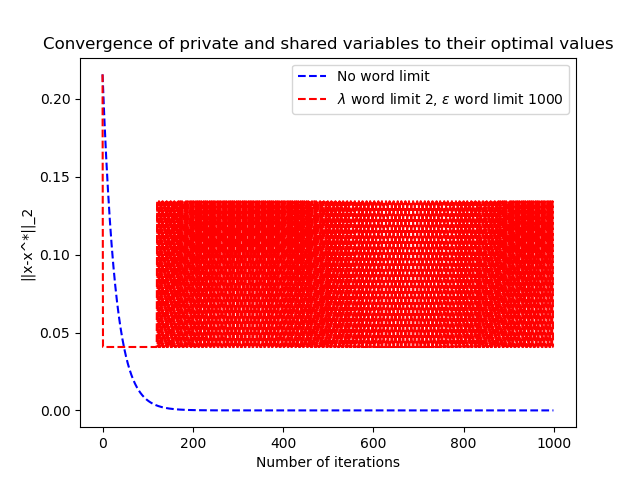
\includegraphics[scale=0.5]{Problem4-Convergence5.png}
	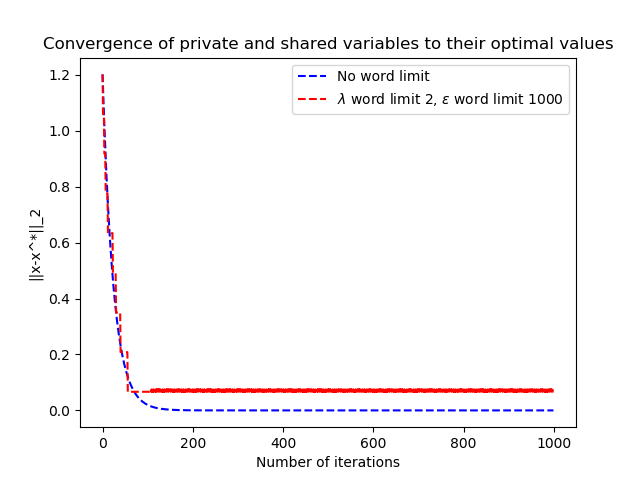
\includegraphics[scale=0.5]{Problem4-Convergence6.png}
	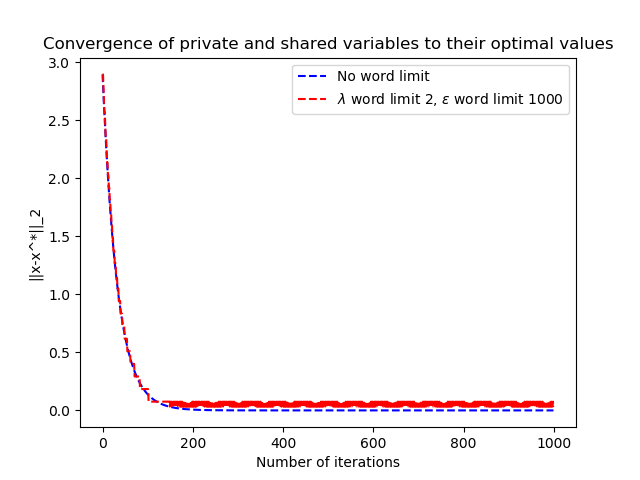
\includegraphics[scale=0.5]{Problem4-Convergence7.png}
	\caption{Convergence for a given limit on $\lambda$ is somewhat dependent on the coefficients of the problem.}
\end{figure}

\begin{figure}[H]
	\centering
	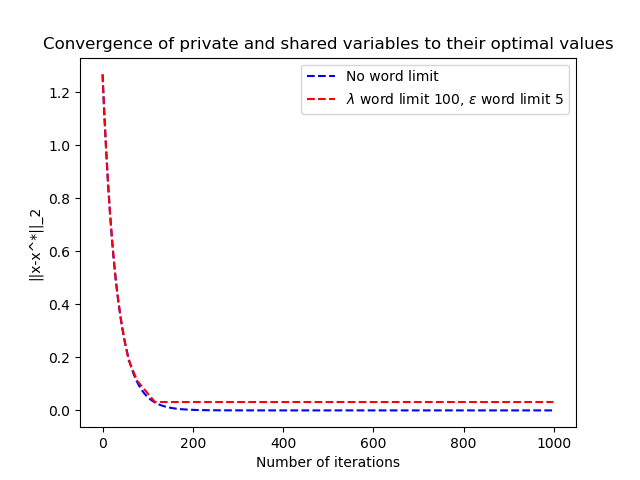
\includegraphics[scale=0.5]{Problem4-Convergence8.png}
	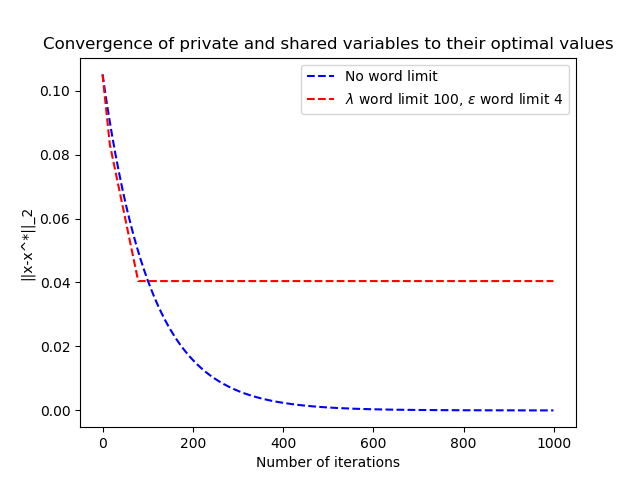
\includegraphics[scale=0.5]{Problem4-Convergence9.png}
	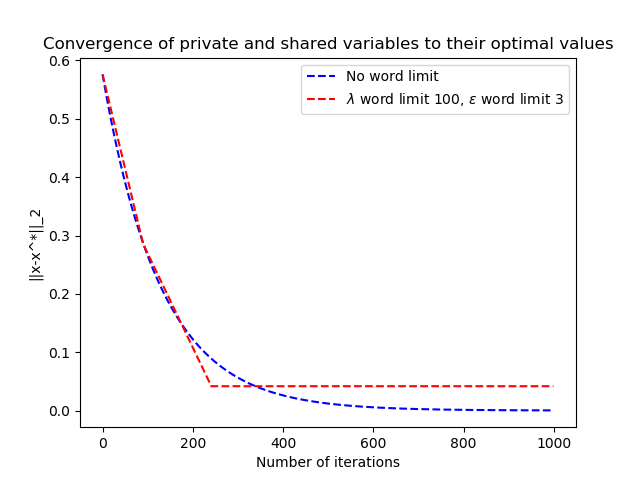
\includegraphics[scale=0.5]{Problem4-Convergence10.png}
	\caption{Similarly, convergence for a given limit on $\xi$ is also somewhat dependent on the randomly generated the problem.}
\end{figure}

Notice for low precision on $\lambda$, the error norm values do not settle at one value in steady state. On the other hand, with low precision on $\xi$ the error does appear to be constant in steady state. Presumably in the case of low precision on $\xi$, it is the rounding error caused by rounding $\xi$ to the closest limited-bit binary representation. Whereas, for low precision on $\lambda$, we enter some limit cycle behaviour when rounding lambda to the closest limited-bit binary representation then recalculation $\xi$, and then reupdating $\lambda$, etc.

\subsection*{How to Run}

\subsubsection*{The above examples}

Make sure you are in the correct directory. Then to run the tests that generated the above plots, execute the \textbf{main.py} file, i.e. use the command

\noindent \textbf{$>>>$python main.py}

Vary lambda\_word\_limit and eps\_word\_limit to generate plots with different binary message limits.

\subsubsection*{Function Descriptions}

The function \textbf{conversions.float2bin}, description.

Syntax: float2bin(number, places)

Parameter values:
\begin{itemize}
	\item number, Required. A float variable that is to be converted to binary representation.
	\item places, Required. Number of bits used to represent the binary fraction of the input number. There is no limit on the number of bits used to represent the binary integer of the input number.
\end{itemize}

Outputs:
\begin{itemize}
	\item Output 1. Binary string representation of the input number. 
\end{itemize}

\noindent The function \textbf{conversions.bin2float}, description.

Syntax: bin2float(bin\_str)

Parameter values:
\begin{itemize}
	\item bin\_str, Required. A binary string representation that is to be converted to float.
\end{itemize}

Outputs:
\begin{itemize}
	\item Output 1. Float representation of input binary string. 
\end{itemize}

\noindent The function \textbf{imprecise.do\_imprecise}, description.

Syntax: do\_imprecise(max\_iter,alpha,A1,A2,b1,b2,xstar,

\qquad\qquad\qquad\qquad lambda\_word\_limit,xi\_word\_limit,verbose=False)

Parameter values:
\begin{itemize}
	\item max\_iter, Required. Number of iterations for the subgradient method.
	\item alpha, Required. Step size for the subgradient method.
	\item A1, Required. The matrix of coefficients $A_1$ as described above.
	\item A2, Required. The matrix of coefficients $A_2$ as described above.
	\item b1, Required. The matrix of coefficients $B_1$ as described above.
	\item b2, Required. The matrix of coefficients $B_2$ as described above.
	\item xstar, Required. True solution to the problem.
	\item lambda\_word\_limit, Required. Word limit of $\lambda$.
	\item xi\_word\_limit, Required. Word limit of $\xi$.
	\item verbose, Default False. Print results to screen.
\end{itemize}

Outputs:
\begin{itemize}
	\item Output 1. The measure of convergence described above, i.e., $||x_{aug}-x^*||_2$.
\end{itemize}

\end{document}